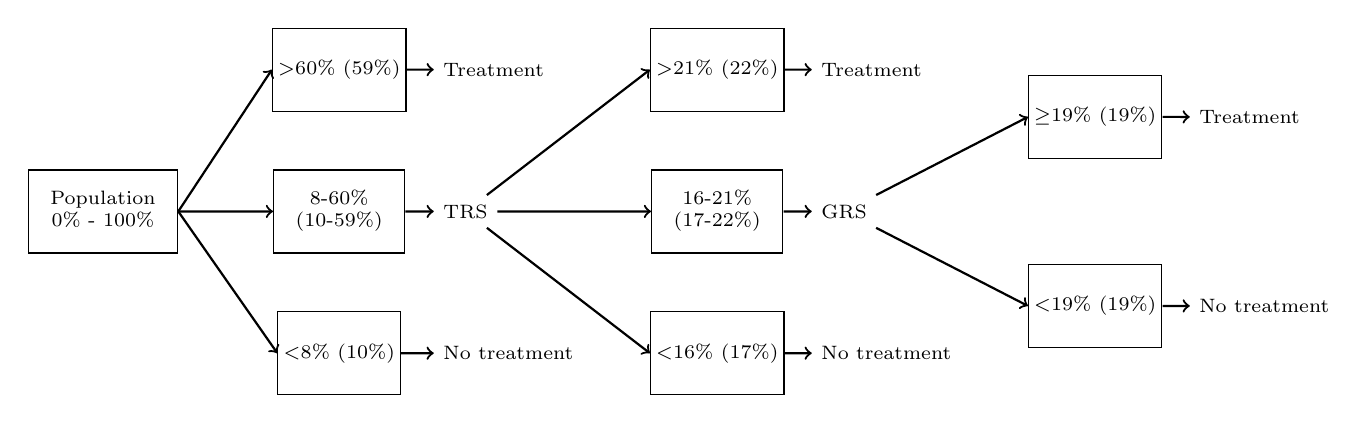
\begin{tikzpicture}
    [decision/.style={draw, minimum size=3em, inner sep=2pt}, 
    scale=1.2]
    % \draw[help lines] (0,0) grid (8,4);
    \node[decision] (1) at (0, 2)  {\scriptsize \begin{tabular}{c} Population \\ 0\% - 100\% \end{tabular}};
    \node[decision] (2) at (2.5, 3.5)  {\scriptsize $>$60\% (59\%)};
    \node[decision] (3) at (2.5, 2)    {\scriptsize \begin{tabular}{c}8-60\% \\ (10-59\%)\end{tabular}};
    \node[decision] (4) at (2.5, 0.5)  {\scriptsize $<$8\% (10\%)};
    \node[right] (T1) at (3.5, 3.5) {\scriptsize Treatment};
    \node[right] (TRS) at (3.5, 2) {\scriptsize TRS};
    \node[right] (NT1) at (3.5, 0.5) {\scriptsize No treatment};
    %
    \node[decision] (5) at (6.5, 3.5)  {\scriptsize $>$21\% (22\%)};
    \node[decision] (6) at (6.5, 2)    {\scriptsize \begin{tabular}{c}16-21\% \\ (17-22\%)\end{tabular}};
    \node[decision] (7) at (6.5, 0.5)  {\scriptsize $<$16\% (17\%)};
    \node[right] (T2) at (7.5, 3.5) {\scriptsize Treatment};
    \node[right] (GRS) at (7.5, 2) {\scriptsize GRS};
    \node[right] (NT2) at (7.5, 0.5) {\scriptsize No treatment};
    %
    \node[decision] (8) at (10.5, 3)  {\scriptsize $\ge$19\% (19\%)};
    \node[decision] (9) at (10.5, 1)  {\scriptsize $<$19\% (19\%)};
    \node[right] (T3) at (11.5, 3) {\scriptsize Treatment};
    \node[right] (NT3) at (11.5, 1) {\scriptsize No treatment};
    %
    \draw[thick, ->] (1.east) -- (2.west);
    \draw[thick, ->] (1.east) -- (3);
    \draw[thick, ->] (1.east) -- (4.west);
    \draw[thick, ->] (2) -- (T1);
    \draw[thick, ->] (3) -- (TRS);
    \draw[thick, ->] (4) -- (NT1);
    \draw[thick, ->] (TRS) -- (5.west);
    \draw[thick, ->] (TRS) -- (6);
    \draw[thick, ->] (TRS) -- (7.west);
    \draw[thick, ->] (5) -- (T2);
    \draw[thick, ->] (6) -- (GRS);
    \draw[thick, ->] (7) -- (NT2);
    \draw[thick, ->] (GRS) -- (8.west);
    \draw[thick, ->] (GRS) -- (9.west);
    \draw[thick, ->] (8) -- (T3);
    \draw[thick, ->] (9) -- (NT3);
\end{tikzpicture}